\documentclass{article}

% Packages
\usepackage[utf8]{inputenc} % For modern characters
\usepackage{microtype} % For sexy kerning
\usepackage{mathtools} % For math stuff
\usepackage{amssymb} % For math symbols
\usepackage{tabularx} % For making tables
\usepackage{fancyhdr} % For headers
\usepackage{pdfpages} % For including a graphics path

% Set the margins to limit the whitespace
\usepackage[scale=0.8, top=1in, bottom=1in]{geometry}

% Other front matter
\graphicspath{ {img/} } % Put all images in img/
\newcommand{\p}[1]{\paragraph{#1}} % Easier to type out for paragraph command
\newcommand{\addsection}[1]{\addcontentsline{toc}{section}{#1}} % content lines
\newcommand{\addsubsection}[1]{\addcontentsline{toc}{subsection}{#1}} % content line
\setcounter{tocdepth}{2} % Set Table of Contents depth
\setlength{\parindent}{0pt} % Disable automatic indentation
\pagestyle{fancy} % Makes header possible
{ %%% Header set up
	\lhead{} % Set the left header to be blank
	\chead{} % Set the center header to be blank
	\rhead{Ben Foster | Homework 7 | June 4, 2015} % Name, assignment, date
}

%%%%%%%%%%%%%%%%%%%%% Begin Document %%%%%%%%%%%%%%%%%%%%%
\begin{document}

{ % Title page, table of contents, and page number setting
	\title{Probability and Statistics for Engineers Homework 7 \\ TMATH 390}
	\author{Ben Foster\thanks{
		Institute of Technology, University of Washington Tacoma} \\
		Instructor: Julia Eaton}
	\date{June 4, 2015} % Include the date
	\maketitle % Make the title
	\thispagestyle{empty} % No page number at the bottom
	\clearpage % Start the table of contents on the next page
	
	\pagenumbering{roman} % Use roman numerals for TOC
	\tableofcontents % Make the table of contents
	\clearpage % Start homework on next page
	\setcounter{page}{1} % Begin numbering over again for HW
	\pagenumbering{arabic} % Use arabic numerals for HW
}

\section*{Problem 1} %%% TODO
\addsection{First Problem}

	State whether each of the following assertions is a legitimate statistical hypothesis and why. \\
	
	(a) H: $\sigma > 100$\\
	(b) H: $\bar{x} = 45$\\
	(c) H: $\tilde{\mu} \not= 2.0$ \\
	(d) H: $s \le 0.50$ \\
	(e) H: $\frac{\sigma_1}{\sigma_2} < 1$ \\
	(f) H: $\bar{x}_1 - \bar{x}_2 = -5.0$ \\
	(g) H: $\lambda < 0.1$, where $\lambda$ is the parameter of an exponential distribution used to 
	model component lifetime. \\
	(h) H: $\pi = 0.10$, where $\pi$ is the population proportion of components that need a warranty 
	service. \\
	(i) H: $x =$ sound of intensity of a certain source (in decibels) has a lognormal distribution.
	
	\addsubsection{Answer to 1.a}
	\p{Answer to a}
	
	\addsubsection{Answer to 1.b}
	\p{Answer to b}
	
	\addsubsection{Answer to 1.c}
	\p{Answer to c}
	
	\addsubsection{Answer to 1.d}
	\p{Answer to d}
	
	\addsubsection{Answer to 1.e}
	\p{Answer to e}
	
	\addsubsection{Answer to 1.f}
	\p{Answer to f}
	
	\addsubsection{Answer to 1.g}
	\p{Answer to g}
	
	\addsubsection{Answer to 1.h}
	\p{Answer to h}
	
	\addsubsection{Answer to 1.i}
	\p{Answer to i}
	
\clearpage
\section*{Problem 2} %%% TODO
\addsection{Second Problem}

	Before agreeing to purchase a large order of polyethylene sheaths for a particular type of high-
	pressure, oil-filled submarine power cable, a company wants to see conclusive evidence that the 
	population standard deviation of sheath thickness is less than 0.05 mm. What hypotheses should 
	be tested, and why? In this context, what are the type I and II errors?
	
	\addsubsection{Answer to 2}
	\p{Answer to 2}

\clearpage
\section*{Problem 3} %%% TODO
\addsection{Third Problem}

	Lightbulbs of a certain type are advertised having an average lifetime of 750 hours. The price of 
	these bulbs is very favorable, so a potential customer has decided to go ahead with a purchase 
	arrangement unless it can be conclusively demonstrated that the true average lifetime is smaller 
	than what is advertised. A random sample of 50 bulbs was selected, the lifetime of each bulb 
	determined, and the appropriate hypotheses were tested using computer software, which gave 
	the following output:
	\begin{center}
	\begin{tabular}{ l r r r r r r }
		Variable & n & Mean & StDev & SEMean & Z & P-Value \\
		lifetime & 50 & 738.44 & 38.20 & 5.40 & -2.14 & 0.016 \\
	\end{tabular}
	\end{center}
	
	(a) Identify the form of the alternative hypothesis used for this problem and justify your answer. \\
	(b) What conclusion would be appropriate at the 0.05 significance level? At the 0.01 significance 
	level?
	
	\addsubsection{Answer to 3.a}
	\p{Answer to a}
	
	\addsubsection{Answer to 3.b}
	\p{Answer to b}

\clearpage
\section*{Problem 4} %%% TODO
\addsection{Fourth Problem}

	To obtain information on the corrosion-resistance properties of a certain type of steel conduit, 35 
	specimens are buried in soil for an extended period. The maximum penetration (in mils) is then is 
	then measured for each specimen, yielding a sample mean penetration of 52.7 and a sample 
	standard deviation of 4.8. The conduits were manufactured with the specification that true 
	average penetration be at most 50 mils. Does the sample data indicate that specifications have 
	not been met? State the relevant hypotheses, calculate the value of the appropriate $z$ statistic, 
	determine the P-value (including a picture of it) and state your conclusion at the 0.05 significance 
	level.
	
	\addsubsection{Answer to 4}
	\p{Answer to 4}

\clearpage
\section*{Problem 5} %%% TODO
\addsection{Fifth Problem}

	A certain pen has been designed so that true average writing lifetime under controlled conditions 
	(involving the use of a writing machine) is at least 10 hours. A random sample of 18 pens is 	
	selected, the writing lifetime of each is determined, and a normal quantile plot of the resulting 
	data supports the use of a one-sample $t$ test. \\
	
	(a) What hypotheses should be tested if the investigators believe a priori that the design 
	specification has been satisfied? \\
	(b) What conclusion is appropriate if the hypotheses of part (a) are tested, $t = -2.3$, and $
	\alpha = .05$? \\
	(c) What conclusion is appropriate if the hypotheses of part (a) are tested, $t = -1.8$, and $\alpha 
	= .01$?
	
	\addsubsection{Answer to 5.a}
	\p{Answer to a}
	
	\addsubsection{Answer to 5.b}
	\p{Answer to b}
	
	\addsubsection{Answer to 5.c}
	\p{Answer to c}

\clearpage
\section*{Problem 6} %%% TODO
\addsection{Sixth Problem}

	Data with $n = 26$ observations on escape time (sec) for oil workers in a simulated exercise, 
	from which the sample mean and sample standard deviation are 370.69 and 24.36, respectively. 
	Suppose the investigators had believed a priori that true average escape time would be at most 6 
	minutes. Do the data contradict this prior belief? Assuming normality, state and test the 
	appropriate hypotheses using a significance level of 0.05.
	
	\addsubsection{Answer to 6}
	\p{Answer to 6}

\clearpage
\section*{Problem 7} %%% TODO
\addsection{Seventh Problem}

	Shoveling is not exactly a high-tech activity but continues to be a required task in our information 
	age. The article ?A Shovel with a perforated blade reduces energy expenditure required for 
	digging wet clay? (\emph{Human Factors}, 2010:492-502) reported on an experiment in which 
	each of 13 workers was provided with both a conventional shovel and a shovel whose blade was 
	perforated with small holes. The authors of the cited article provided the following data on stable 
	energy expenditure (measured in kilocalories per kg of subject per pounds of clay): \\
	
	\iffalse
	%\begin{center}
	\newgeometry{textwidth=10cm, textheight=10cm}
	\begin{tabular}{ l c c c c c c c c c c c c c }
		Worker & 1 & 2 & 3 & 4 & 5 & 6 & 7 & 8 & 9 & 10 & 11 & 12 & 13 \\
		Conventional & 0.0011 & 0.0014 & 0.0018 & 0.0022 & 0.0010 & 0.0016 & 0.0028 & 0.0020 
		& 0.0015 & 0.0023 & 0.0017 & 0.0020 & 0.0014 \\
		Perforated & 0.0011 & 0.0010 & 0.0019 & 0.0013 & 0.0011 & 0.0017 & 0.0024 & 0.0020 & 
		0.0013 & 0.0017 & 0.0020 & 0.0013 & 0.0013 \\
	\end{tabular}
	\restoregeometry
	%\end{center}
	\fi
	
	\begin{center}
		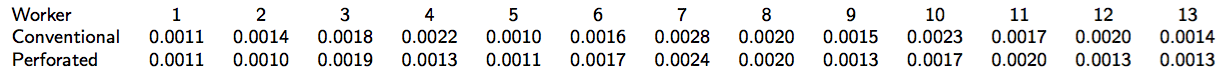
\includegraphics[width=\textwidth]{Prob7.jpg}
	\end{center}
	
	Carry out a test of hypotheses at significance level 0.05 to see whether the true average energy 
	expenditure using the conventional shovel exceeds that using the perforated shovel.
	
	\addsubsection{Answer to 7}
	\p{Answer to 7}

\clearpage
\section*{Problem 8} %%% TODO
\addsection{Eighth Problem}

	Which factors are relevant to the time a consumer spends looking at a product on the shelf prior 
	to selection? The article ?Effects of Base Price Upon Search Behavior of Consumers in a 
	Supermarket? (\emph{J. Econ. Psycho.}, 2003: 637-652) reported the following data on elapsed 
	time (sec) for fabric softener purchasers and washing0up liquid purchasers; the former product is 
	significantly more expensive than the latter. These products were chosen because they are 
	similar with respect to allocated shelf space and number of alternative brands.
	
	\begin{center}
	\begin{tabular}{ l c c c }
		\textbf{Product} & \textbf{sample size} & \textbf{sample mean} & \textbf{sample std.dev.} \\
		Fabric softener & 15 & 30.47 & 19.15 \\
		Washing-up liquid & 18 & 26.53 & 15.37 \\
	\end{tabular}
	\end{center}
	
	(a) What, if any, assumptions, are needed before the $t$ inferential procedure can be used to 
	compare true average elapsed times? \\
	(b) Carry out a test of hypotheses to decide whether the true average differences in elapsed time 
	differs from zero.
	
	\addsubsection{Answer to 8.a}
	\p{Answer to a}
	
	\addsubsection{Answer to 8.b}
	\p{Answer to b}

\clearpage
\section*{Problem 9} %%% TODO
\addsection{Ninth Problem}

	Sample observations on stabilized viscosity of asphalt specimens are (2781, 2900, 3013, 2856, 
	and 2888). For a particular application, it is required that true average viscosity be 3000. Does 
	this requirement appear to have been satisfied? State and test the appropriate hypotheses at 
	significance level 0.05.
	
	\addsubsection{Answer to 9}
	\p{Answer to 9}

\clearpage
\section*{Problem 10} %%% TODO
\addsection{Tenth Problem}

	Criminologists have long debated whether there is a relationship between weather and violent 
	crime. The author of the article ?Is There a Season for Homicide?? (\emph{Criminology}, 1988: 
	287-296) classified 1361 homicides according to season, resulting in the data below:
	
	\begin{center}
	\begin{tabular}{ l c c c c }
		\textbf{Season:} & Winter & Spring & Summer & Autumn \\
		\textbf{Frequency:} & 328 & 334 & 372 & 327 \\
	\end{tabular}
	\end{center}
	
	Does the data suggest that the homicide rate somehow depends on the season? State the 
	relevant hypotheses, then carry out the hypothesis test at the 5\% significance level.
	
	\addsubsection{Answer to 10}
	\p{Answer to 10}

\clearpage
\section*{Problem 11} %%% TODO
\addsection{Eleventh Problem}

	A random sample of individuals who drive to work in a large metropolitan area was obtained, and 
	each individual was categorized according to commuting distance (in miles):
	
	\begin{center}
	Commuting distance \\
	\begin{tabular}{ l l | c c c } \\ \hline
		& & Low & Medium & High \\
		& & [0 mi, 10 mi) & [10 mi, 20 mi) & [20 mi, $\infty$) \\ \hline
		Type of vehicle & subcompact & 6 & 27 & 19 \\
		& compact & 8 & 36 & 17 \\
		& full-size & 14 & 18 & 6 \\
	\end{tabular}
	\end{center}
	
	Does the data suggest that there is an association between type of vehicle and commuting 
	distance? State the appropriate hypotheses and carry out the test using a significance level of 
	0.05.
	
	\addsubsection{Answer to 11}
	\p{Answer to 11}

\end{document}